%Florian Bogner
%e1225415
%Optimierung der Anzahl der Ausbildungstellen im österreichischen Gesundheitssystem
%Bacc-Seminar

\documentclass[a4paper,12pt]{article}
\usepackage{fullpage}
\usepackage[utf8]{inputenc}
\usepackage[ngerman]{babel}
\usepackage{amsmath}
\usepackage{amssymb}
\usepackage{latexsym}
\usepackage{mathtools}
\usepackage{listings}
\usepackage{algorithm}
\usepackage{algpseudocode}
\usepackage{graphicx}

\begin{document}

\begin{titlepage}
\huge
\centering
Optimierung der Anzahl der Ausbildungstellen im österreichischen Gesundheitssystem 

\vfill

\normalsize
Florian Bogner

Betreut von: Claire Rippinger \& Christoph Urach
%oder whs der Breitenegger
\end{titlepage}




\tableofcontents
\newpage

\section{Abstract}

\section{Einleitung}



\subsection{Das Modell}

Es handelt sich um ein agentenbasiertes Modell. Die Agenten repräsentieren ÄrztInnen an verschiedenen Stellen in ihrer Ausbildung oder ihrem Berufsleben. Sie beginnen als Studenten an einer der sieben Universitäten für Medizin in Österreich. Nach dem Studienabschluss beginnen die Agenten mit ihrem Turnus, entweder als Allgemeinmediziner (AM) oder Facharzt (FA). Absolventen der AM-Ausbildung entscheiden sich dann ob sie als AM berufstätig werden oder die FA-Ausbildung beginnen. 

Die Ausbildung im Turnus und das Berufsleben ist aufgeteilt auf die neun Bundesländer und weiter aufgeteilt auf den Urbanisationsgrad (Städte, Kleinstädte und Vororte, Ländliche Gebiete). Die Agenten treffen während ihrer Laufbahn viele Entscheidungen wie z.B. Studienwechsel, Emigration, Wahl der Ausbildungsstelle, Berufswechsel, Vollzeit oder Teilzeit, etc. 

Das ganze Modell hat hunderte Parameter, die zum größten Teil aus Expertenschätzungen bestehen oder aus historischen Daten extrapoliert wurden. Der Anfangszustand besteht aus aktuellen echten Daten. Das Modell wird dann bis zu einem festgelegtem Jahr durchgerechnet und Informationen über alle Agenten in Form einer Datenbank gespeichert. Aus dieser kann man dann alles auslesen, was man beobachten will.

\begin{figure}[h]
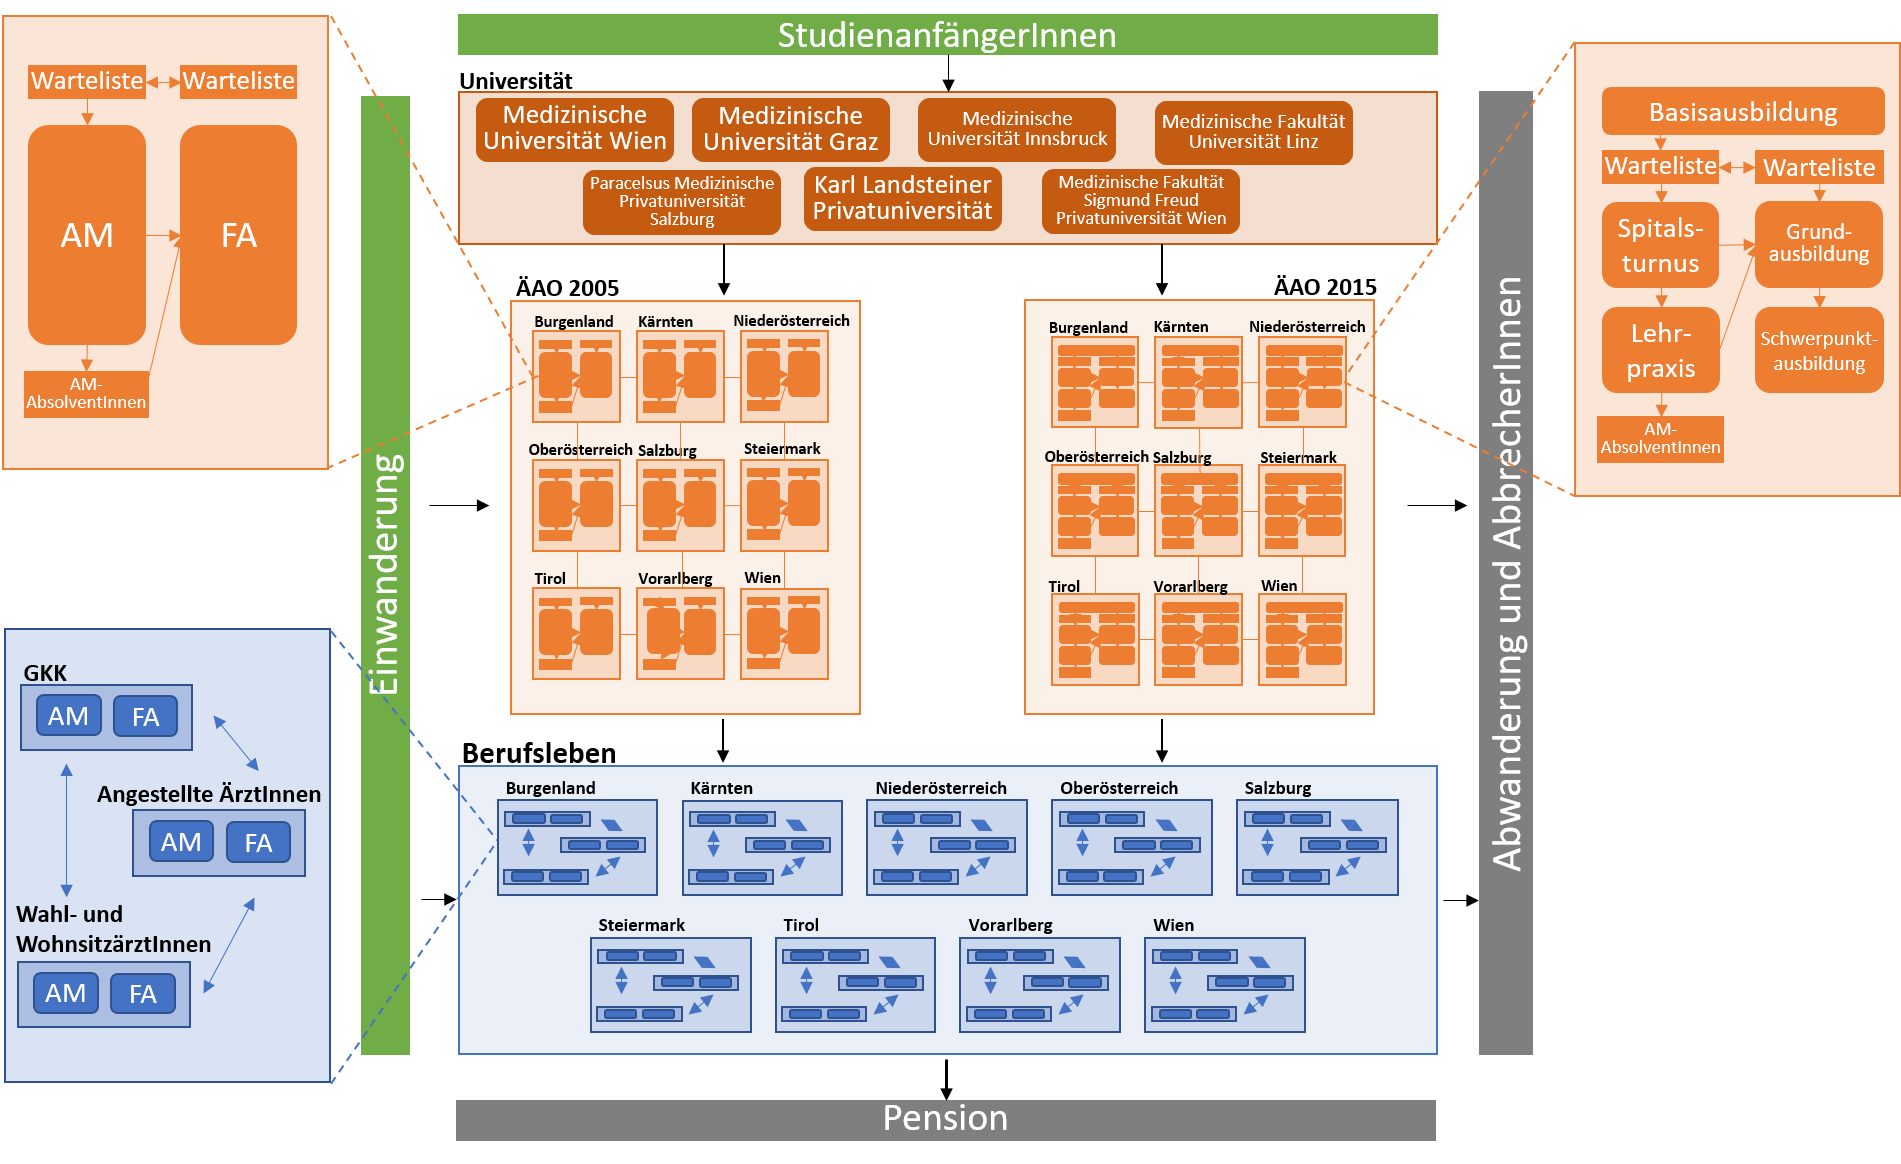
\includegraphics[width=\textwidth]{modellgraph.png}
\caption{Karrierestationen der Agenten im Modell}
\end{figure}


\subsection{Die Aufgabestellung}

%Jedes Jahr gehen ÄrztInnen in Pension. Die offenen Stellen, die dadurch hinterlassen werden, sollen idealerweise durch Berufseinsteiger möglichst genau gefüllt werden. Um dies zu erzielen, müssen die Anzahlen der Ausbildungsstellen jedes Jahr genau gewählt werden. Mit dieser optimalen Wahl beschäftigt sich diese Seminararbeit.

Diese Seminararbeit beschäftigt sich mit der optimalen Wahl der Anzahl der Ausbildungsstellen, jeweils für Allgemeinmediziner und Fachärzte. Jedes Jahr, wenn ÄrztInnen in Pension gehen, werden offene Stellen hinterlassen, die idealerweise durch Berufseinsteiger gefüllt werden. Ziel ist es, genau so viele Absolventen wie offene Stellen in den jeweiligen Bereichen zu haben.

\subsection{Das vereinfachte Modell}

Es wird keine Rücksicht auf das Bundesland, in dem ein angehender Arzt seine Ausbildung absolviert, sowie die Fachrichtung eines angehenden Facharztes genommen. Es werden nur die Anzahl der freien Stellen und Absolventen aller Fachrichtungen in ganz Österreich verglichen. Die Anzahl der Ausbildungsstellen werden für je drei Jahre konstant angenommen. Dies bewirkt eine Dimensionsreduktion im Parameterraum.

\newpage

\section{Kalibrierungsansätze}

Das Problem verlangt nach Algorithmen, die nur mit Funktionsauswertungen auskommen und keine Gradienten oder Richtungsableitungen brauchen, da die Parameter des Modells ja natürliche Zahlen sind und numerische Gradientenbestimmung sowieso zu teuer wäre.

Die drei verwendeten Algorithmen haben einiges gemeinsam. Als gemeinsame Argumente haben sie eine Funktion $f: \mathbb{R}^d \rightarrow \mathbb{R}$, die Dimension $d$ und eine Matrix $bounds = \binom{a_1, \cdots, a_d}{b_1, \cdots, b_d} \in \mathbb{R}^{2\times d}$, die einen Quader $\bigtimes\nolimits_{i=1}^d [a_i, b_i] \subset \mathbb{R}^d$ beschreibt. Aus diesem Quader werden die Startwerte gewählt. Das gesuchte Minimum sollte in diesem Quader sein. 

Als Output haben die Algorithmen (natürlicherweise) den Input für die Funktion $f$ wo das Minimum vermutet ist. 

Durch die unmittelbare Anwendungsnähe ist Echtzeit-Laufzeit das wichtigste Bewertungskriterium. Durch die moderne Prozessorarchitektur mit mehreren Kernen betrachten wir auch die Parallelisierbarkeit der Algorithmen. Da die Verwendung von mehreren Kernen in einem Simulationsdurchlauf nicht einfach möglich ist, bzw. nicht im Scope dieser Seminararbeit liegt müssen wir uns mit der parallelen Ausführung von mehreren Simulationsdurchläufen begnügen.

\subsection{Partikelschwarm}

Dieser Algorithmus basiert auf einem Schwarm von Partikeln die sich durch den Parameterraum bewegen. Zu Beginn des Algorithmus werden die Positionen von einer Anzahl an Partikeln innerhalb der $bounds$ sowie deren Geschwindigkeit zufällig gewählt. In jedem Schritt wird die Geschwindigkeitsänderung, also eine Beschleunigung ausgerechnet. Diese zieht die Partikel zum Teil zu dem bisher besten Punkt, den der jeweilige Partikel erreicht hat und zum Teil zum bisher besten Punkt überhaupt. Zur Geschwindigkeit wird dann jeweils die Beschleunigung addiert und zur Position die Geschwindigkeit. 

\begin{algorithm}
\caption{Partikelschwarm}
\begin{algorithmic}
\Function{findminimum}{$f,d,bounds, numOfParticles, maxV, acc$}\\

%pos = randomly selected from $bounds^{numOfParticles}$\\
%vel = randomly selected direction\\

$I := \{1,2,\hdots,numOfParticles\}$\\
$(pos_i)_{i\in I} =$ Vektor von zufällig gewählten Positionen innerhalb der $bounds$\\
$(vel_i)_{i\in I} =$ Vektor von zufällig gewählten Richtungen\\

$pBest_i = \infty$\\
$gBest = 1$\\

\While{}

\EndWhile	
\EndFunction	
\end{algorithmic}
\end{algorithm}


%\lstinputlisting[language=python, firstline = 52 , lastline = 98]{../particleswarm.py}

Der Partikelschwarm-Algorithmus eignet sich hervorragend zu Parallelisierung. Die Partikel bewegen sich alle gemeinsam in einem Zeitschritt und deren neue Position muss danach gleichzeitig ausgewertet werden. Idealerweise wählt man dann auch noch die Anzahl der Partikel als ein Vielfaches der Anzahl der verfügbaren Prozessorkerne um alle Kerne immer zu nutzen.

\subsection{Sintflut}

Der Sintflut-Algorithmus ist eine Verbesserung des naiven Hill-Climbing-Algorithmus, welcher an einem zufälligen Punkt im Parameterraum startet und dann iterativ zufällige Schritte macht. Bei einer Verbesserung wird der neue Punkt angenommen, sonst bleibt man beim alten Punkt. Eine große Schwäche des Hill-Climbing-Algorithmus ist das leichte Verfangen in lokalen Optima. Der Sintflut-Algorithmus verspricht diese Schwäche zu korrigieren.

Bildlich gesprochen befindet sich ein herumirrender Wanderer in einer Landschaft mit Hügeln und Tälern.\footnote{Für die bildliche Vorstellung suchen wir jetzt das Maximum, nicht das Minimum wie oben angegeben} Es regnet konstant und so steigt der Wasserspiegel immer weiter an. Der Wanderer, anders als im Hill-Climbing-Algorithmus kann jetzt auch bergab gehen, aber er kann nicht schwimmen. Wenn der Wanderer schließlich keinen Schritt mehr machen kann, ohne nasse Füße zu bekommen, muss er wohl einen Gipfel erreicht haben. Durch die Möglichkeit bergab zugehen erhofft man sich die gröbere Toleranz gegenüber lokalen Optima.

\begin{algorithm}
\caption{Sintflut}
\begin{algorithmic}
\Function{findminimum}{$f, d, bounds, Sealevel, Rain, Schrittweite, (optional) Startparameter$}\\



\EndFunction	
\end{algorithmic}
\end{algorithm}

Die Wahl des Startwasserstands und der Regenmenge ist von großer Bedeutung. Bei zu tiefen Wasserstand wandert man unbeschränkt herum und verschwendet effektiv Rechenzeit, oder schlimmer sogar wandert weit weg vom (z.B. als gute Schätzung gewählten) Startwert. Bei zu hohem Wasserstand startet der Wanderer vielleicht schon in mitten eines Ozeans, weit weg von Land. Der Algorithmus bricht dann schnell ohne Ergebnis ab.

Die Regenmenge kontrolliert quasi die Konvergenzrate. Bei zu viel Regen kann der Wanderer vielleicht nicht schnell genug auf einen Berg flüchten. Je weniger Regen, desto länger dauert die Ausführung des Algorithmus, doch die Genauigkeit und die Konfidenz in das Ergebnis steigt.

In der originalen Quelle\footnote{TODO: Ordentliche Quellenangaben und Zitate} ist nur von einer kleinen stochastischen Änderung die Rede. Welche Verteilung diese haben soll wird nicht näher spezifiziert. Eine naheliegende Möglichkeit ist die Normalverteilung mit $\mu = 0$ und $\sigma$ als kleinen Wert der als Schrittweitenparameter betrachtet werden kann.\footnote{Der Wanderer ist dann ein Wiener.} Eine andere Möglichkeit ist eine feste Schrittweite in eine zufällige Richtung zu gehen. Letztlich wurde eine Affinkombination dieser beiden gewählt. 

%%% Normalverteilung, normierte Normalverteilung (also konstanter Schrittweite in zufällige Richtung, deren Linearkombination (also die Tischtuch über Donut-Verteilung) %%%

Durch die einzelnen Schritte eignet sich dieser Algorithmus nicht besonders gut zur Beschleunigung durch Parallelisierung. Man kann spekulativ mehrere mögliche Schritte zugleich auswerten und, falls der erste ins Wasser steigt, den zweiten überprüfen und so weiter. Man erkauft sich dadurch ein bisschen Beschleunigung, aber viele der Auswertungen fließen gar nicht in den Algorithmus ein. Mit steigender Prozessorkernanzahl trifft man schnell auf diminishing returns. 



\subsection{Downhill Simplex}

Dieser Algorithmus basiert auf einem Simplex im Parameterraum, also der konvexen Hülle von $d+1$ vielen Punkten. Die Eckpunkte werden ausgewertet und in jedem Schritt wird der schlechteste Eckpunkt durch einen (hoffentlich) besseren ersetzt. Der Simplex bewegt sich dadurch im Laufe der Zeit dem figurativen Hügel hinab einem lokalen Minimum entgegen und zieht sich letztendlich über dem Minimum zusammen.

\begin{algorithm}
\caption{Downhill Simplex}
\begin{algorithmic}
\Function{findminimum}{$f, d, bounds, \alpha = 1, \gamma = 2, \beta = \frac{1}{2}, \sigma = \frac{1}{2}$}

\State $x_i$ für $i \in \mathbb{N}_{\leq d}$ werden zufällig innerhalb der $bounds$ gewählt

\For{$k \in \mathbb{N}_{< totalSteps}$}

\State sortiere $x_i$ sodass $f(x_0) < f(x_1) < \hdots < f(x_d)$

\State $m := \frac{1}{d} \sum^{d-1}_{i = 0} x_i$ \Comment{der Mittelpunkt aller Ecken außer der schlechtesten}

\State $r := (1+\alpha)m - \alpha x_d$ \Comment{Reflexion von $x_d$ an $m$}

\If{$f(r) < f(x_0)$}

\State $e := (1+\gamma)m - \gamma x_d$ \Comment{Der Expandierte Punkt}

\If{$f(e) < f(r)$}

\State $x_d := e$

\Else

\State $x_d := r$

\EndIf

\ElsIf{$f(r) < f(x_{d-1})$}

\State $x_d := r$

\Else

\If{$f(r) < f(x_N)$}

\State $h := r$

\Else

\State $h := x_N$

\EndIf

\State $c := \beta m  + (1-\beta) h$

\If{$f(c) < f(x_d)$} \Comment{Der Kontrahierte Punkt}

\State $x_d := c$

\Else

\State $x_i := \sigma x_0 + (1-\sigma) x_i) \forall i \neq 0$ \Comment{Komprimiere den Simplex}

\EndIf

\EndIf

\EndFor
\EndFunction	
\end{algorithmic}
\end{algorithm}

Im Pseudocode wurde $f$ hier oftmals zur Klarheit doppelt und dreifach aufgerufen. In der tatsächlichen Implementation wird $f$ für jeden Punkt natürlich nur einmal aufgerufen und das Ergebnis gespeichert. In jedem Schritt gibt es zwei Möglichkeiten, entweder der schlechteste Punkt wird ersetzt oder der Simplex wird komprimiert. Zweiteres tritt dann auf, wenn keiner der 


\subsection{Vergleich}

\newpage

\section{Bewertungsfunktionen}

\subsection{Die erste Bewertungsfunktion}

Die folgenden Variablen sind allesamt Vektoren, die die jeweilige Größe für Allgemeinmediziner ($AM$) und Fachärzte ($FA$) über die Simulationsperiode $J$ darstellen.

\begin{center}
\begin{tabular}{ | c | c | l | r |}
\hline
$AM_a$ & $FA_a$ & gesamte Ausbildungsstellen & Modellparameter \\ \hline
$AM_o$ & $FA_o$ & offen gebliebene Ausbildungsstellen & Modellresultat \\ \hline
$AM_f$ & $FA_f$ & Berufseinsteiger (f wie fertig) & Modellresultat \\ \hline
$AM_p$ & $FA_p$ & pensionierte Ärzte & vorgegebener Zielwert \\ \hline
\end{tabular}
\end{center}

Die erste Bewertungsfunktion ist:

\begin{align*}
F_1(\hdots) = 	c_1 &\cdot \left\| \frac{(AM_f - AM_p)}{AM_p} \cdot (1, \cdots, 0.5)  \right\|_2 + \\
			c_2 &\cdot \left\| \frac{(FA_f - FA_p)}{FA_p} \cdot (1, \cdots, 0.5)  \right\|_2  +\\
			c_3 &\cdot \left\| \left( \frac{ \sum\nolimits_{j=1}^i AM_{f,j} - AM_{p,j} }{\sum\nolimits_{j=1}^i AM_{p,j} } \right)_{i\in J} \right\|_2 +\\
			c_4 &\cdot \left\| \left( \frac{ \sum\nolimits_{j=1}^i FA_{f,j} - FA_{p,j} }{\sum\nolimits_{j=1}^i FA_{p,j} } \right)_{i\in J} \right\|_2 +\\
			c_5 &\cdot \left\| \frac{AM_o}{AM_a} \right\|_2 +\\
			c_6 &\cdot \left\| \frac{FA_o}{FA_a} \right\|_2 
\end{align*}

wobei die Divisionen und die Multiplikationen als komponentenweise zu verstehen sind. Die ersten beiden Terme bestrafen Abweichungen zum Zielwert, also die Diskrepanz zwischen Berufseinsteigern und Pensionierten. Dies ist mit einer Diskontierung versehen, um Abweichungen in naher Zukunft stärker zu gewichten wie Abweichungen gegen Ende der untersuchten Periode. 

Die zweiten zwei Terme bestrafen kumulierten Fehler. Betrachten wir folgende Beispiele: 1) In einem Jahr gibt es 200 Anfänger zu wenig, im darauffolgenden Jahr 200 zu viel. 2) In beiden Jahren sind 200 Anfänger zu wenig. Beide Beispiele werden von den ersten beiden Termen gleich bewertet, doch in der Realität ist das erste Beispiel wünschenswerter, da die Lücken vom ersten Jahr ja im Nächsten gefüllt werden. 

Die dritten zwei Komponenten bestrafen offene Ausbildungsstellen. Dies ist offensichtlich davon motiviert, keine Ressourcen zu verschwenden.

Die Koeffizienten $\vec c$ wurden anfänglich als $(1,1,1,1,2,2)$ gewählt und dies scheint keine schlechte Wahl gewesen zu sein.

%
%\subsection{Der Zielbereich der ersten  Bewertungsfunktion}
%
%Der Fehler besteht aus 6 Summanden, die jeweils aus 12 (1-4) oder 15 (5-6) Summanden besteht. Jeder Term hier liegt zwischen und 0 und ungefähr 1. Ein Summand kann größer als 1 sein, falls zum Beispiel mehr als doppelt so viele Jungärzte fertig werden wie pensioniert werden, also sehr selten.
%
%Das Minimum der Fehlerfunktion ist also 0. Es wird erreicht, wenn alle Lücken durch Pensionierungen genau gefüllt werden und alle Ausbildungsplätze besetzt sind. Ideal, aber unrealistisch.

\subsection{Die zweite Bewertungsfunktion}

Die zweite Bewertungsfunktion ist eine Erweiterung der ersten:

\begin{align*}
F_2(\hdots) =	F_1&(\hdots) \hspace{4pt} + \\
			c_7 &\cdot \sum\limits_{i\in J\backslash\{1\}} \left( \frac{AM_{a,i-1} - AM_{a,i} }{1000} \right) ^ 4 + \\
			c_8 &\cdot \sum\limits_{i\in J\backslash\{1\}} \left( \frac{FA_{a,i-1} - FA_{a,i} }{1000} \right) ^ 4
\end{align*}

Nach ein paar Testläufen ist aufgefallen, das immer wieder Lösungen gefunden werden, in denen die Anzahl der Ausbildungsstellen stark schwingt. Dies ist natürlich unrealistisch, da zum Beispiel viele Ausbildungsplätze schaffen, nur um den Großteil davon in 3 Jahren wieder abzuschaffen ist eine Verschwendung von Ressourcen. Deshalb wurde die erste Fehlerfunktion um weitere zwei Terme erweitert, die große Sprünge bestraft. 

Der Koeffizienten $\vec c$ wurden auf $(1,1,1,1,2,2,2,2)$ erweitert. 

\subsection{Die dritte Bewertungsfunktion}

Im Laufe des Testens ist aufgefallen, dass manchmal im Laufe eines Downhill-Simplex-Algorithmus die Anzahl der Ausbildungsstellen divergieren.\footnote{Die vermeintlichen Lösungen entsprechen freiem Zugang zu Ausbildungsstellen, welcher vielleicht die beste Lösung zum Problem des Ärztemangels wäre.} Nachdem lange erfolglos ein Fehler im Algorithmus gesucht wurde, wurde klar, dass der Fehler in der Bewertungsfunktion liegt. In der fünften und sechsten Komponente steht der Anteil an unbesetzten Ausbildungsstellen. Ob dieser nun 99\% oder 99.9\% ist, macht nur ein winzigen Unterschied für die Bewertungsfunktion,  aber entspricht (bei gleich vielen Auszubildenden) einer zehnfachen Erhöhung der Ausbildungsstellen. Zur Korrektur wird auf die betreffenden Terme eine Funktion angewandt, die in der Nähe der $0$ ähnlich wie die Identität ausschaut \footnote{Diese Bedingung sorgt dafür, dass $F_2 \leq F_3$ immer und $F_2 \approx F_3$ bei kleinen Anteilen der unbesetzten Ausbildungsstellen.} und bei $1$ gegen $\infty$ konvergiert.

\begin{equation*}
f: [0,1) \rightarrow [0,\infty) : x \mapsto \frac{x}{1-x}
\end{equation*}

erfüllt diese Eigenschaften und die dritte Bewertungsfunktion lautet somit:

\begin{align*}
F_3(\hdots) = \hdots & \hspace{4pt} + \\
			c_5 &\cdot \left\| f\left( \frac{AM_o}{AM_a} \right) \right\|_2 +\\
			c_6 &\cdot \left\| f\left( \frac{FA_o}{FA_a} \right) \right\|_2 +\\
			 \hdots &
\end{align*}


%\section{Technische Details}
%
%Die gesamte Codebase ist in Python 3 geschrieben. 

\section{Resultate}

\section{Fazit}



\end{document}
































